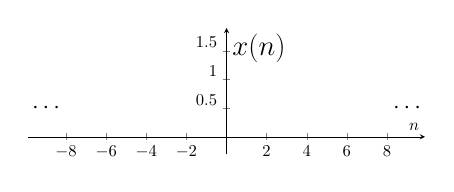
\begin{tikzpicture}[scale=0.6,transform shape]
    \begin{axis}[
        x=0.035\textwidth,y=0.1\textwidth,
    	axis y line=center,
    	axis x line=middle,
    	xlabel=$n$,ylabel={\LARGE $x(n)$},
    	xmin=-9.9,xmax=9.9,
    	ymin=-0.3,ymax=1.9,
    	xticklabel style = {xshift=0},
    	yticklabel style = {yshift=5},
    	]
    	\discretedelta{-8}{0.1};
    	\discretedelta{-7}{0.1};
    	\discretedelta{-6}{1};
    	\discretedelta{-5}{1};
    	\discretedelta{-4}{1};
    	\discretedelta{-3}{1};
    	\discretedelta{-2}{0.1};
    	\discretedelta{-1}{0.1};
    	\discretedelta{0}{1};
    	\discretedelta{1}{1};
    	\discretedelta{2}{1};
    	\discretedelta{3}{1};
    	\discretedelta{4}{0.1};
    	\discretedelta{5}{0.1};
    	\discretedelta{6}{1};
    	\discretedelta{7}{1};
    	\discretedelta{8}{1};
    	\node at (-9,0.5) {\Large $\cdots$};
    	\node at (9,0.5) {\Large $\cdots$};
    \end{axis}
\end{tikzpicture}